\chapter{Elastic Linear Plates}

\modinfo{Module name}{Smitc}
\modinfo{Module subroutines}{\Idx{SmitcSolver}}
\begin{versiona}
\modinfo{Module authors}{Mikko Lyly, Jani Paavilainen}
\modinfo{Document authors}{Mikko Lyly, Peter R�back}
\modinfo{Document created}{August 26th 2002}

\def\curv{\underline{\underline\kappa}}
\def\mom{\underline{\underline m}}
\def\G{\underline{\underline \nabla}}
\def\Id{\underline{\underline I}}

\section{Introduction}

The linear elastic plate elements of Elmer are based on the shear deformable
model of Reissner and Mindlin.The finite element discretization is performed
using the so called stabilized MITC-plate elements, which are free from
numerical locking.

\subsection{Reissner-Mindlin model}

The displacement $\vec u = (u_x, u_y, u_z)$ of a Reissner-Mindlin
plate (thin or moderately thick linearly elastic body which in its
undeformed reference configuration occupies the three dimensional
region $\Omega \times(-{t\over 2},{t\over 2})$, where $\Omega$ is
the midsurface and $t$ the thickness) is obtained from the kinematic
equations
\begin{eqnarray}
&& u_x(x,y,z) = -\theta_x(x,y) \cdot z \label{plateux} \\ && u_y(x,y,z) =
-\theta_y(x,y) \cdot z \label{plateuy} \\ && u_z(x,y,z) = w(x,y)
\label{plateuz}
\end{eqnarray}
where $\theta_x$ and $\theta_y$ are components of the rotation
vector $\underline\theta=(\theta_x, \theta_y)$ and $w$ is the
transverse deflection of the mid-surface, see Figure 1.

The functions $w$ and $\underline\theta=(\theta_x, \theta_y)$ are
determined from the condition that they minimize the total
potential energy
\begin{equation}
{1\over 2}\int_\Omega \curv : \mom \ d\Omega + \int_\Omega
\underline\gamma \cdot \underline q \ d\Omega - \int_\Omega pw \
d\Omega\label{linplateenergy}
\end{equation}
where $p$ is the transverse pressure load, $\curv = {1\over 2}
(\G\underline\theta + \G\underline\theta^T)$ is the curvature of
the mid-surface, $\underline \gamma = \underline\nabla w -
\underline\theta$ is the transverse shear strain, $\mom =
{\mathcal E}:\curv$ is the bending moment, and $\underline q =
{\mathcal G}\cdot\underline\gamma$ the transverse shear force
vector. The fourth order tensor $E$ and second order tensor $\mathcal G$
define the bending and shear rigidities of the cross section, respectively.
For linearly elastic materials we have $\mathcal G \cdot \underline
\gamma = Gt \underline\gamma$ and
\begin{equation}
\mathcal E : \curv =  K [\curv + {\nu \over 1-\nu} (tr \curv) \Id]
\end{equation}
where $K={Et^3 /[ 12(1-\nu^2) ]}$ is the bending stiffness, $E$ is
Young's modulus, $G$ shear modulus, and $\nu$ Poisson ratio. The
design of the tensors $\mathcal E$ and $\mathcal G$ for orthoropic
and perforated materials is discussed in section \ref{reikasysteemi}.

The minimizer of the energy satisfies the equilibrium equations
\begin{eqnarray}
&& \underline\nabla \cdot \mom + \underline q = 0 \label{momeq} \\ && - \nabla
\cdot\underline q = p \label{sheareq}
\end{eqnarray}

\subsection{Surface tension}

When surface tension is present, the following term is added to
the energy:
\begin{equation}
{1\over 2}\int_\Omega \underline\nabla w \cdot {\mathcal T}
\cdot\underline\nabla w \ d\Omega
\end{equation}
where $\mathcal T$ is a second order tensor representing the given
normal force (usually $\mathcal T = T \Id$, where $T$ is constant).
The equilibrium equation (\ref{sheareq}) is then rewritten as
\begin{eqnarray}
 && - \nabla \cdot(\underline q + \mathcal T \cdot \nabla w) = p 
\label{sheqt} 
\end{eqnarray}


\subsection{Boundary conditions}

The following boundary conditions can be applied in the
Reissner-Mindlin plate model:
\begin{itemize}
\item Soft fixed edge: $w=0$ and $\underline \theta\cdot\underline n = 0$
\item Hard fixed edge: $w=0$ and $\underline \theta = \underline 0$
\item Soft simply supported edge: $w=0$
\item Hard simply supported edge: $w=0$ and $\underline\theta \cdot \underline
t = 0$
\item Free edge: $\mom \cdot \underline n = 0 $ and $(\underline q + \mathcal T\cdot\underline\nabla w)\cdot \underline  n = 0 \label{bcqn}$
\end{itemize}
The boundary conditions can of course be non-homogenous as well.
For fixed and simply supported edges the prescribed values of $w$,
$\underline\theta$, $\underline \theta \cdot\underline n$, and
$\underline\theta\cdot\underline t$, are taken into account on
matrix level after finite element discretization. On the free part
of the edge, the non-homogenous case is trated by adding the following
terms in the energy:
\begin{equation}
\int_{\Gamma_{free}} q_n w \ d\Gamma + \int_{\Gamma_{free}} \underline m_n
\cdot\underline\theta \ d\Gamma
\end{equation}
where $q_n = \underline q\cdot\underline n$ and $\underline m_n = 
\mom \cdot\underline n$ are prescribed functions.

\subsection{Kirchhoff plates}

When the thickness of the plate is small ($t << \rm{diam}
(\Omega)$), the Reissner-Mindlin model can be considered
as a penalty approximation of the classical plate model
of Kirchhoff. The Kirchhoff model is obtained from
(\ref{plateux})-(\ref{sheqt})
by enforcing the constraint $\underline\gamma = \underline 0$.
The governing equations are then reduced to
\begin{equation}
K\Delta \Delta w - T \Delta w = p \label{kplate}
\end{equation}

\subsection{Transient and natural mode analysis}

A transient plate model is obtained by adding the interia term
$\rho t \ddot w$ on the left hand-side of (\ref{sheareq}), (\ref{sheqt}),
and (\ref{kplate}). Here $\rho$ is the density of the material. The
natural vibration frequencies and mode shapes are then obtained by taking
$p=0$ and solving the Fourier transformed equations.

\section{Finite element implementation}

The direct minimization of (\ref{linplateenergy}) using the standard
Galerkin finite element
method fails due to the well known numerical locking phenomena 
(the method is unable to deal with the Kirchhoff constraint $\underline
\gamma = \underline 0$, which becomes valid when $t$ is small). In
order to avoid locking, Elmer utilizes the so called SMITC (Stabilization
and Mixed Interpolation of Tensorial Components) elements, which are
known to be optimally convergent and work well under all conditions
\cite{ls94}.

The linear element of the SMITC-family was first introduced by
Brezzi, Fortin and Stenberg in \cite{bfs}.  The method is defined by
replacing the shear energy term in (\ref{linplateenergy}) by the
following numerical modification:
\begin{equation}
\int_\Omega \underline\gamma_h \cdot \underline q_h \ d\Omega
\end{equation}
where $\underline\gamma_h$ is called the reduced shear strain
(sometimes also referred to as the assumed or substitute shear)
and $\underline q_h = (t^2 + \alpha h^2)^{-1} \mathcal G \cdot
\underline \gamma_h$ the reduced shear force. Here $h$ is the
mesh size (the diameter of the biggest element) and $\alpha>0$
is a numerical stabilization parameter (typically $\alpha = 0.15$).

The reduced shear $\underline\gamma_h$ is defined elementwise
such that
\begin{equation}
\underline\gamma_{h|K} = ( a_K - b_K y,  a_K + c_K x)
\end{equation}
for any element $K$. The parameters $a_K,b_K$, and $c_K$, are
determined from the conditions
\begin{equation}
\int_E (\underline\gamma - \underline\gamma_h)\cdot\underline t \ ds = 0
\end{equation}
for every edge $E$ of $K$. Here $\underline t$ is the counterclockwise
tangent to $E$.


It has been shown~\cite{lyly} that the linear SMITC-element is equivalent
to the T3BL (Triangle, 3 nodes, Linked Interpolation) element of Xu, Auricchio
and Taylor \cite{xu,at95}, the anisoparametrically interpolateed MIN3 element
of Tessler and Hughes \cite{th85}, and the TRIA3 element of MacNeal
\cite{macneal}. We refer to \cite{lyly} for a more detailed discussion.

\section{Elastic parameters for \Idx{perforated plate}s}
\index{energy method}\label{reikasysteemi}

In microelectromechanical systems the plate stuctures are often perforated 
in order to reduce the squeezed-film damping effect. This has also an
effect on the elasticity equation. If there are so many holes that it is not feasible 
to treat them individually their effect may be homogenized over the whole 
structure. In practice this means that the original elastic parameters are replaced by
\Idx{effective parameters} that take into account the holes. 
This method was reported by Pedersen et al.~\cite{pedersen1} and
implemented into the solver by Jani Paavilainen.

\index{ortotropic}
In the homogenization effective parameters for an ortotropic plate 
are defined so that the unperforated model approximates the 
perforated plate.
The basic idea is to set the analytical expressions of the 
deformation energies of the 
perforated and unperforated plates equal. This method is 
inherently limited to simple geometries where analytical expressions may be found.
So far, only square holes have been implemented in the solver.

\begin{figure}[tbhp]
\vspace{-5cm}
\centerline{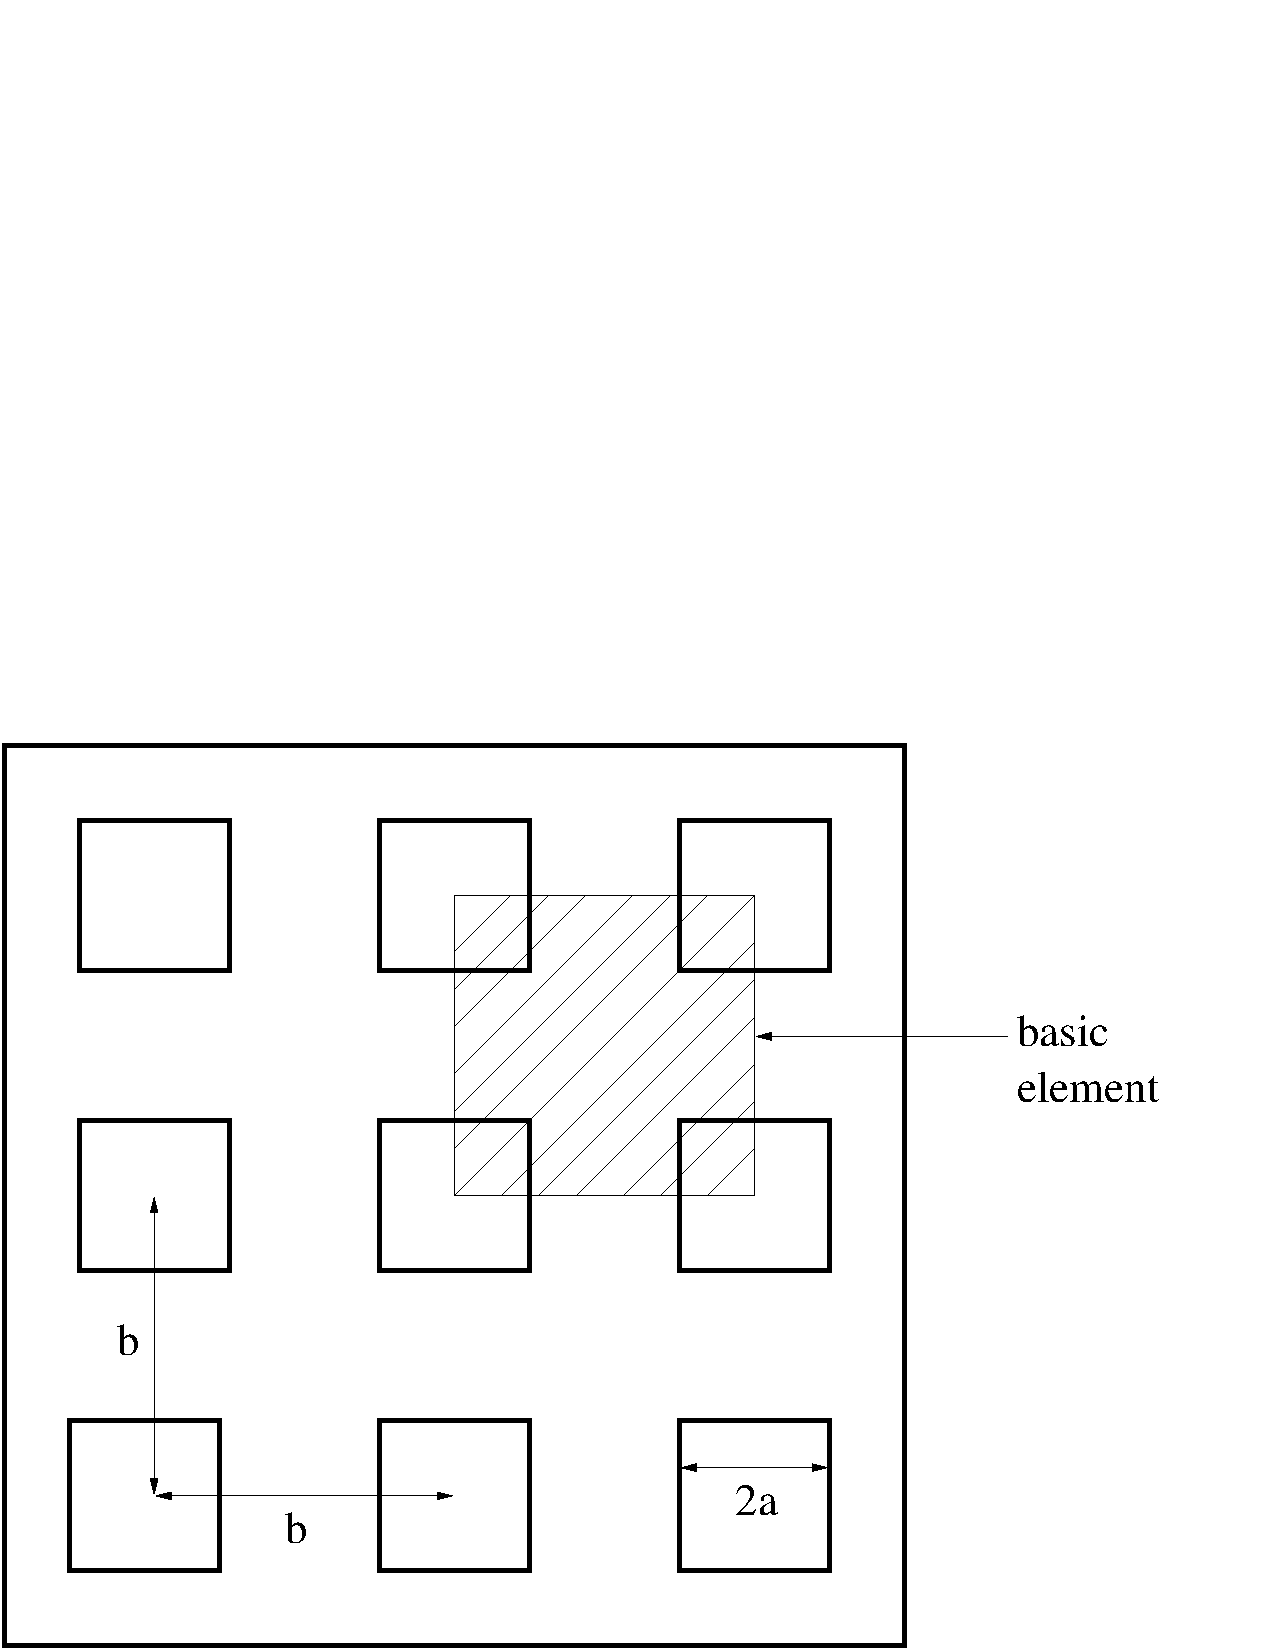
\includegraphics[width=0.6\textwidth]{basic-element}}
\caption{The basic element of the perforated plate consisting of five rectangular
beams}
\label{fg:basic}
\end{figure}

The unit cell of a perforated plate may be assumed to consist of one 
small square plate with side $b-2a$, and of four beams of length $a$ as
shown in Figure~\ref{fg:basic}.
Using approximate formulas an analytical formula for the deformation
energy of the perforated plate is obtained.  
This has to be equal to the deformation energy of 
an unperforated ortoropic membrane. From this condition we get a set of equations
from which the effective parameters may be solved.

The elasticity tensor has three independent components, 
$C_{11}=C_{22}, C_{12}=C_{21}$, and $C_{44}$. 
The expressions for these are
~\cite{pedersen1},
\begin{eqnarray}
C_{11} & = & C_{22} = \frac{E}{b^{2}} \left \{ \frac{b(b-2a)}{1-\nu^{2}} + 
\frac{a(b-2a)^{2}}{b} \right \} \label{eq:C1} \\
C_{12} & = & C_{21} = \frac{\nu E (b-2a)}{b(1- \nu^{2})} \label{eq:C2} \\
C_{44} & = & \frac{E}{4b^{2}(1+ \nu)} \left \{ 2b(b-2a) + \frac{12 K a(b-2a)}{bh^{3}} 
\right\}. \label{eq:C3}
\end{eqnarray} 
where $K$ is a constant\footnote{In article~\cite{pedersen1} there is an error in the definition of
$K$. In the article there is an expression $(b-2a)/h^{3}$, which would make $K$ 
discontinuous at $h=b-2a$.}, 
defined as
\begin{equation}
K= \left \{ \begin{array}{ll}
\frac{1}{3} \left (1-0.63 \frac{b-2a}{h} \right)(b-2a)^{3}h, \quad \mbox{jos  }h>b-2a \\
\frac{1}{3} \left (1-0.63 \frac{h}{b-2a} \right)(b-2a)h^{3}, \quad \mbox{jos  }h<b-2a.  
\end{array}
\right.
\end{equation}

The midplane tension of the perfomarated plate may be reduced to 
lateral stresses of the ortotropic plate by a simple scaling, 
\begin{equation}
 T = \sqrt{(1-4a^{2}/b^{2})} \, T_0 , \label{eq:sigmared}
\end{equation}
where is the tension $T_0$ of the perforated plate. Using this reduced tension and
the modified material parameters of equations~(\ref{eq:C1}),~(\ref{eq:C2}) and~(\ref{eq:C3}) 
the ortoropic plate mimics the behavior of the perforated plate 
when looking at macroscopic quantities. However, the model is not suitable for approximating
maximum stresses around the holes, for example.

\section{Keywords}
\end{versiona}

\sifbegin
\sifitemnt{Solver}{solver id}
\sifbegin
\sifitemnt{Equation}{String SmitcSolver}
\sifitem{Variable}{String Deflection}
This may be of any name as far as it is used consistently also elsewhere.
\sifitem{Variable DOFs}{Integer 3}
Degrees of freedom for the deflection. 
The first degree is the displacment and the two following ones
are its derivatives in the direction of the coordinate axis.
\sifitem{Eigen Analysis}{Logical}
Also the eigenvalues and eigenmodes of the elasticity equation may be computed.
This is done automatically by calling a eigensolver after the original equation has been solved.
The default is \texttt{False}.
\sifitem{Eigen System Values}{Integer}
If the eigenvalues are computed this keyword gives the number of eigenmodes
to be computed. The lowest eigenvalues are always solved for.
\sifitem{Hole Correction}{Logical} 
If the plate is perforated the holes may be taken into account by 
a homogenized model. This is activated with this keyword.
The default is \texttt{False}.
\sifitemnt{Procedure}{File "Smict"\ "SmitcSolver"}
\sifend

\sifitemnt{Material}{mat id}
\sifbegin
\sifitem{Density}{Real}
Density of the plate.
\sifitemnt{Poisson ratio}{Real}
\sifitem{Youngs modulus}{Real}
The elastic parameters are given with Youngs modulus and Poisson ratio.
\sifitem{Thickness}{Real}
Thickness of the plate.
\sifitem{Tension}{Real}
The plate may be pre-stressed.
\sifitemnt{Hole Size}{Real}
\sifitem{Hole Fraction}{Real}
If \texttt{Hole Correction} is \texttt{True} the solver 
tries to find the size and relative fraction of the holes. 
If these are present the hole is assumed to be a square hole.
\sifend

\sifitemnt{Boundary Condition}{bc id}
\sifbegin
\sifitem{Deflection i}{Real}
Dirichlet BC for the components of the deflection, i=1,2,3.
\sifitem{Current Density BC}{Logical}
Must be set to {\tt True} if Neumann BC is used.
\sifitem{Current Density}{Real}
Neumann boundary condition for the current.
\sifend

\sifitemnt{Body Force}{bf id}
\sifbegin
\sifitem{Pressure}{Real}
Possibility for a body forces. For coupled systems there is a 
possibility to have up to three forces. The two others are then
marked with \texttt{Pressure B} and \texttt{Pressure C}.
\sifitem{Spring}{Real}
The local spring which results to a local force when multiplyed
by the displacement.
\sifitem{Damping}{Real}
The local damping which results to a local force when multiplyed
by the displacement velocity. The spring and damping may also be 
defined as material parameters.
\sifend

\sifend


\begin{versiona}
\bibliography{elmerbib}
\bibliographystyle{plain}
\end{versiona}
